\documentclass[a4paper,12pt]{article}
\usepackage{bbding,combelow,textcomp,amsfonts,amsthm,amsmath,amssymb,graphicx,color,hyperref,etoolbox}
\usepackage[utf8x]{inputenc}
\usepackage[lined,boxed,commentsnumbered]{algorithm2e}
\usepackage{float}
\usepackage{booktabs}
\usepackage{tikz}
\usetikzlibrary{arrows.meta,positioning,calc,fit,backgrounds}

\newtoggle{story}


%%%%%%%%%%%%%%%%%%%%%%%%%%%%%%%%%%%%%%%%%%
%% Customisation options --- update as necessary
%%%%%%%%%%%%%%%%%%%%%%%%%%%%%%%%%%%%%%%%%%

%% Course details: title, semester, instructors

\newcommand{\courseTitle}{Combinatorics II (Math 7702)}
\newcommand{\semester}{Spring 2026}
\newcommand{\instructorA}{Shagnik Das}
\newcommand{\instructorB}{Lu Yun-Chi}

%% Sheet number

\newcommand{\sheetNumber}{4}


%% Submission details

\newcommand{\dueDate}{15:30, May 26th.}
\newcommand{\lateWarning}{Late submissions will receive no credit.}


%% Display irrelevant footnotes?  \toggletrue for yes, \togglefalse for no

\toggletrue{story}

%%%%%%%%%%%%%%%%%%%%%%%%%%%%%%%%%%%%%%%%%%
%% End of customisation options
%%%%%%%%%%%%%%%%%%%%%%%%%%%%%%%%%%%%%%%%%%

\pdfpagewidth 8.5in
\pdfpageheight 11in
\topmargin -1in
\headheight 0in
\headsep 0in
\textheight 8.5in
\textwidth 6.5in
\oddsidemargin 0in
\evensidemargin 0in
\headheight 77pt
\headsep 0in
\footskip .75in

\makeatletter
\newcommand{\buildtitle}[4]{
\begin{flushleft}
{\large
#1
\hfill{}
#2
\par
#3
}
\end{flushleft}
\vskip 4pt
\begin{center}
{\large\bfseries#4\par}
\end{center}
\bigskip
}
\makeatother

\renewcommand{\thesection}{\normalsize\arabic{section}}

\renewcommand{\deg}{\textrm{deg}}
\newcommand{\eps}{\varepsilon}
\newcommand{\ceil}[1]{\left \lceil #1 \right \rceil}

\newcommand{\hint}{\begin{flushright} [Hint at \url{\hintURL}.] \end{flushright}}

\newcommand{\card}[1]{\left| #1 \right|}
\newcommand{\mb}[1]{\mathbb{#1}}
\newcommand{\mc}[1]{\mathcal{#1}}


\newcommand{\story}[1]{\iftoggle{story}{\footnote{#1}}{}}
\newcommand{\storymark}[1][42]{\iftoggle{story}{\footnotemark[#1]}{}}
\newcommand{\storytext}[2][42]{\iftoggle{story}{\footnotetext[#1]{#2}}{}}

\newcommand{\bonus}[2]{\paragraph{Bonus (#1 pt\ifstrequal{#1}{1}{}{s})} #2}


\begin{document}


\buildtitle{\courseTitle{}}{\semester}{\instructorA{} \hfill \instructorB{}}{Exercise Sheet \sheetNumber{}}

\vspace{-0.2in}

\begin{center}

{B13902024 Chang, Yi-Kuei \\ \bf Due date: \dueDate \\ \lateWarning}

\end{center}

\noindent You should try to solve all of the exercises below, and then submit two solutions to be graded --- each problem is worth $10$ points. Make sure to clearly justify your answers, defining everything precisely and stating any results you are using. You should then submit your solutions on NTU COOL, either as a typed PDF or a clear picture or scan of your handwritten answers.

\paragraph{Exercise 1}  Table 1 provides the capacities along the edges of a network. Find a flow of maximum possible value from Madrid (`Mad') to the British Virgin Islands (`BVI'), and give a short proof that one cannot do better.

\begin{table}[h!] \label{tab:capacities}
\center
\begin{tabular}{|ccc|c||ccc|c|}
	\hline
	Start & $\rightarrow$ & End & Capacity (\$, mil) & Start & $\rightarrow$ & End & Capacity (\$, mil) \\ \hline
	Mad & $\rightarrow$ & Ams & 50 & Mad & $\rightarrow$ & Dub & 140 \\ 
	Ams & $\rightarrow$ & Jer & 40 & Ams & $\rightarrow$ & Lux & 40 \\
	Ams & $\rightarrow$ & Ber & 50 & Jer & $\rightarrow$ & Lux & 30 \\
	Dub & $\rightarrow$ & Ams & 130 & Dub & $\rightarrow$ & Z\"ur & 20 \\
	Dub & $\rightarrow$ & Cay & 50 & Ber & $\rightarrow$ & Dub & 60 \\
	Ber & $\rightarrow$ & Z\"ur & 60 & Lux & $\rightarrow$ & Ber & 40 \\
	Lux & $\rightarrow$ & Z\"ur & 30 & Lux & $\rightarrow$ & BVI & 60 \\
	Cay & $\rightarrow$ & Z\"ur & 30 & Z\"ur & $\rightarrow$ & BVI & 120 \\ \hline
\end{tabular}
\caption{The capacities along the edges of a network.}
\end{table}

\paragraph{Solution:}
A maximum flow has value $170$.  One such flow is shown below; each edge label
has the form $f/c$, where $f$ is the flow on that edge and $c$ is its capacity.

\begin{center}
\resizebox{\textwidth}{!}{%
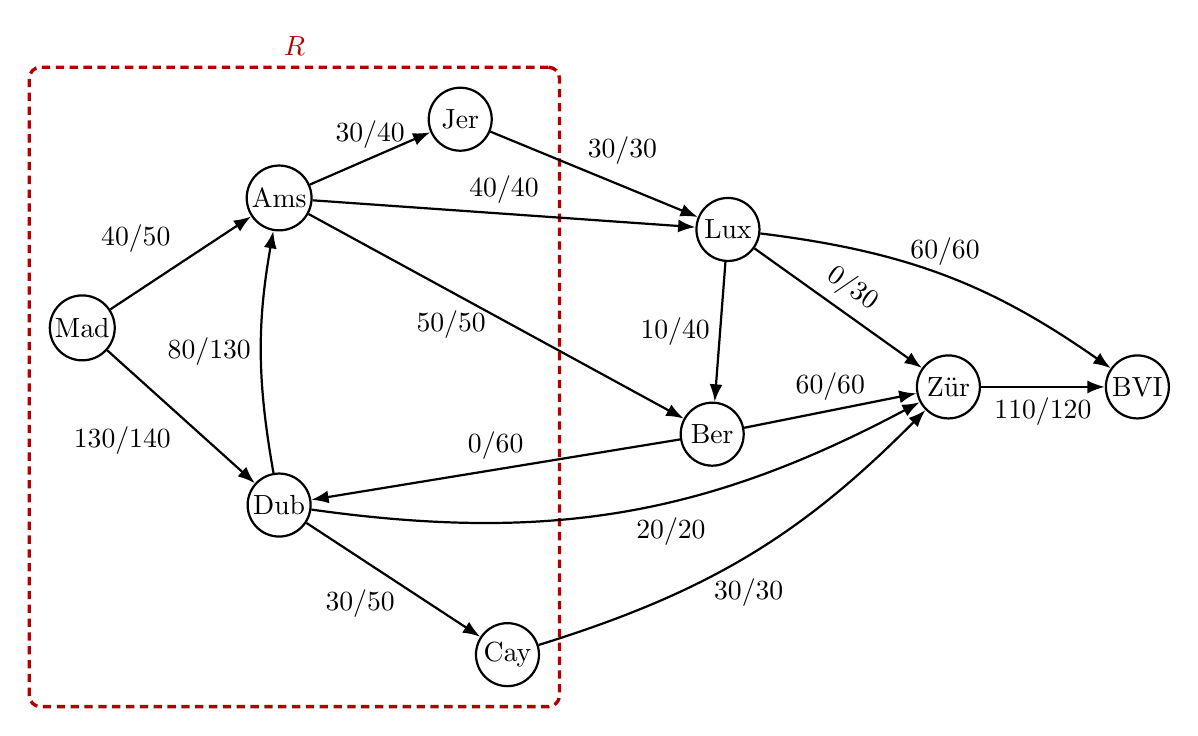
\begin{tikzpicture}[
    x=1cm,y=1cm,
    city/.style={circle,draw,thick,minimum size=8mm,inner sep=1pt,fill=white},
    edge/.style={-{Latex[length=2.2mm]},thick},
    cut/.style={densely dashed,very thick,red!70!black},
    cutset/.style={draw=red!70!black,densely dashed,very thick,rounded corners,inner sep=7pt}
]
\node[city] (Mad) at (0,0) {Mad};
\node[city] (Ams) at (2.5,1.65) {Ams};
\node[city] (Dub) at (2.5,-2.25) {Dub};
\node[city] (Jer) at (4.8,2.65) {Jer};
\node[city] (Cay) at (5.4,-4.15) {Cay};
\node[city] (Lux) at (8.2,1.25) {Lux};
\node[city] (Ber) at (8.0,-1.35) {Ber};
\node[city] (Zur) at (11.0,-0.75) {Z\"ur};
\node[city] (BVI) at (13.4,-0.75) {BVI};

\draw[edge] (Mad) -- node[above left] {$40/50$} (Ams);
\draw[edge] (Mad) -- node[below left] {$130/140$} (Dub);
\draw[edge] (Ams) -- node[above] {$30/40$} (Jer);
\draw[edge] (Ams) -- node[above] {$40/40$} (Lux);
\draw[edge] (Ams) -- node[left, yshift=-3pt] {$50/50$} (Ber);
\draw[edge] (Jer) -- node[above right, xshift=-6pt] {$30/30$} (Lux);
\draw[edge,bend left=10] (Dub) to node[left] {$80/130$} (Ams);
\draw[edge] (Dub) -- node[below, xshift = -12pt] {$30/50$} (Cay);
\draw[edge,bend right=18] (Dub) to node[below,pos=0.58,yshift=-2pt] {$20/20$} (Zur);
\draw[edge] (Ber) -- node[above] {$0/60$} (Dub);
\draw[edge] (Ber) -- node[above] {$60/60$} (Zur);
\draw[edge] (Lux) -- node[left] {$10/40$} (Ber);
\draw[edge] (Lux) -- node[above,sloped] {$0/30$} (Zur);
\draw[edge,bend left=14] (Lux) to node[above] {$60/60$} (BVI);
\draw[edge,bend right=14] (Cay) to node[below, yshift=-5pt] {$30/30$} (Zur);
\draw[edge] (Zur) -- node[below] {$110/120$} (BVI);

\begin{scope}[on background layer]
\node[cutset,fit=(Mad) (Ams) (Dub) (Jer) (Cay),label={[red!70!black]above:$R$}] {};
\end{scope}
\end{tikzpicture}%
}
\end{center}

The corresponding edge flows are:
\[
\begin{array}{c|c@{\qquad}c|c}
\text{edge} & f & \text{edge} & f \\ \hline
\text{Mad}\to\text{Ams} & 40 & \text{Mad}\to\text{Dub} & 130 \\
\text{Ams}\to\text{Jer} & 30 & \text{Ams}\to\text{Lux} & 40 \\
\text{Ams}\to\text{Ber} & 50 & \text{Jer}\to\text{Lux} & 30 \\
\text{Dub}\to\text{Ams} & 80 & \text{Dub}\to\text{Z\"ur} & 20 \\
\text{Dub}\to\text{Cay} & 30 & \text{Ber}\to\text{Dub} & 0 \\
\text{Ber}\to\text{Z\"ur} & 60 & \text{Lux}\to\text{Ber} & 10 \\
\text{Lux}\to\text{Z\"ur} & 0 & \text{Lux}\to\text{BVI} & 60 \\
\text{Cay}\to\text{Z\"ur} & 30 & \text{Z\"ur}\to\text{BVI} & 110
\end{array}
\]
All listed flows are at most their capacities.  Flow is also conserved at each
intermediate vertex: for example, Ams receives $40+80=120$ and sends
$30+40+50=120$, while Z\"ur receives $20+60+0+30=110$ and sends $110$.
The value of the flow is therefore
\[
40+130=170,
\]
the total flow leaving Mad, equivalently $60+110=170$, the total flow entering
BVI.

It remains to show that no larger flow is possible.  Consider the cut
\[
R=\{\text{Mad},\text{Ams},\text{Dub},\text{Jer},\text{Cay}\},
\qquad
V\setminus R=\{\text{Lux},\text{Ber},\text{Z\"ur},\text{BVI}\}.
\]
The edges directed from $R$ to $V\setminus R$ are
\[
\text{Ams}\to\text{Lux},\quad
\text{Ams}\to\text{Ber},\quad
\text{Jer}\to\text{Lux},\quad
\text{Dub}\to\text{Z\"ur},\quad
\text{Cay}\to\text{Z\"ur}.
\]
Their total capacity is
\[
40+50+30+20+30=170.
\]
Every feasible flow is bounded above by the capacity of every source--sink cut,
so no flow can have value more than $170$.  Since the displayed feasible flow
has value $170$, the maximum possible flow is
\[
\boxed{170\text{ million dollars}}.
\]

\paragraph{Exercise 2}
\begin{itemize}
	\item[(a)] If $G$ is $k$-connected, and $G'$ is obtained by adding a new vertex $v$ of degree at least $k$, show that $G'$ is also $k$-connected.
	\item[(b)] Prove that $G$ is $k$-connected if and only if it has at least $k+1$ vertices and, for any two sets $A, B \subset V(G)$ of size $k$, there are $k$ pairwise-disjoint paths\footnote{Note that a path could consist of just a single vertex.} that start in $A$ and end in $B$.
\end{itemize}

\paragraph{Solution:}
\begin{enumerate}
    \item[\textbf{(a)}]
    We want to show that for any subset $S \subseteq V(G')$ with $|S| < k$, the graph $G' - S$ is connected. We consider two cases based on whether the new vertex $v$ is removed:
    
    \medskip
    \noindent\textbf{Case 1:} $v \in S$. \\
    In this case, removing $S$ from $G'$ is equivalent to removing $S \setminus \{v\}$ from $G$. That is,
    \[
    G' - S = G - (S \setminus \{v\})
    \]
    Since $|S| < k$, it follows that $|S \setminus \{v\}| < k - 1 < k$. Because $G$ is $k$-connected, removing fewer than $k$ vertices from $G$ leaves it connected. Thus, $G - (S \setminus \{v\})$ is connected, which implies $G' - S$ is connected.
    
    \medskip
    \noindent\textbf{Case 2:} $v \notin S$. \\
    Since $v \notin S$, we can view $G' - S$ as the graph $G - S$ with the vertex $v$ (and its remaining incident edges) added back. 
    Because $G$ is $k$-connected and $|S| < k$, the graph $G - S$ is connected. 
    Furthermore, we are given that $\deg_{G'}(v) \ge k$. Since $|S| \le k - 1$, the vertex $v$ loses at most $k - 1$ neighbors when $S$ is removed. Therefore, in $G' - S$, the vertex $v$ retains at least:
    \[
    \deg_{G'-S}(v) \ge k - |S| \ge 1
    \]
    neighbor. Since $G - S$ is connected and $v$ has at least one neighbor in $G - S$, the graph $G' - S$ remains connected.
    
    \medskip
    Since $G' - S$ is connected in both cases, $G'$ is $k$-connected.

    \item[\textbf{(b)}]

    $(\Rightarrow)$ Assume $G$ is $k$-connected and $|V(G)| \ge k+1$. Let $A, B \subseteq V(G)$ be any two subsets of size $k$. 
    
    We construct an auxiliary graph $G^*$ by adding two new vertices $s$ and $t$ to $G$, such that $s$ is connected to all vertices in $A$, and $t$ is connected to all vertices in $B$. 
    Since $\deg(s) = k$ and $\deg(t) = k$, applying the result from part \textbf{(a)} twice guarantees that $G^*$ remains $k$-connected.
    
    By the local-vertex version of Menger's Theorem, since $s$ and $t$ are non-adjacent vertices in a $k$-connected graph, there exist $k$ internally vertex-disjoint paths between $s$ and $t$ in $G^*$. 
    Each of these $k$ paths must be of the form $s - a_i - \dots - b_i - t$, where $a_i \in A$ and $b_i \in B$. By deleting the endpoints $s$ and $t$ from each path, we obtain $k$ paths in $G$ that start in $A$ and end in $B$. Since the original paths were internally disjoint, these $k$ resulting paths in $G$ must be pairwise vertex-disjoint.
    
    \medskip
    $(\Leftarrow)$ Assume $|V(G)| \ge k+1$ and for every $A, B \subseteq V(G)$ with $|A| = |B| = k$, there exist $k$ pairwise-disjoint paths starting in $A$ and ending in $B$. We show by contradiction that $G$ is $k$-connected.
    
    Suppose $G$ is not $k$-connected. Then there exists a separating set $S \subset V(G)$ with $|S| < k$ such that $G - S$ is disconnected. We can expand $S$ to a set $S'$ of size exactly $k-1$ by arbitrarily adding $k - 1 - |S|$ vertices from the remaining components. Since $|V(G)| \ge k+1$, removing $S'$ leaves at least two vertices, and $G - S'$ remains disconnected.
    
    Let $C_1$ and $C_2$ be two distinct connected components of $G - S'$. Choose an arbitrary vertex $x \in C_1$ and $y \in C_2$. Now, construct two sets $A$ and $B$ of size $k$ as follows:
    \[
    A = \{x\} \cup S' \quad \text{and} \quad B = \{y\} \cup S'
    \]
    Note that $|A| = |B| = k$ because $x, y \notin S'$. 
    
    By our initial assumption, there must exist $k$ pairwise-disjoint paths from $A$ to $B$. Since these $k$ paths are pairwise vertex-disjoint, each of the $k-1$ vertices in $S'$ can belong to at most one path. Therefore, at most $k-1$ of these paths can contain any vertex from $S'$.
    
    Since there are $k$ paths in total, at least $k - (k-1) = 1$ path must be completely free of any vertices in $S'$. This path must begin at the only remaining vertex of $A$ (which is $x$) and end at the only remaining vertex of $B$ (which is $y$). 
    
    Consequently, this path lies entirely within $G - S'$, establishing a connection between $x \in C_1$ and $y \in C_2$. This directly contradicts the fact that $C_1$ and $C_2$ are disconnected components in $G - S'$. 
    
    Thus, $G$ must be $k$-connected.
\end{enumerate}

\paragraph{Exercise 3}  Consider the network in the figure below. The source and the sink are marked with $S$ and $T$, and the capacities of all but one edge are indicated. The remaining edge has capacity $\frac12(\sqrt{5} - 1)$.


\begin{itemize}
	\item[(a)] Find (with proof) the value of the maximum flow in the network.
	\item[(b)] Describe a choice of augmenting paths in the Ford-Fulkerson algorithm for which the algorithm never finishes and the flow value converges to $2+\sqrt{5}$.
\end{itemize}

\paragraph{Exercise 4}  The goal of this exercise is to prove the local, vertex version of Menger's Theorem; that is, given a graph $G$ and non-adjacent vertices $x, y \in V(G)$, $\kappa(x,y) = \lambda(x,y)$.  We construct a directed graph $\vec{D}$ with vertices $V(\vec{D}) = \{ v^+, v^- : v \in V(G) \}$ and edges $\vec{E}(\vec{D}) = \{ (u^+, v^-), (v^+, u^-) : uv \in E(G) \} \cup \{ (v^-, v^+) : v \in V(G) \}$.  We then assign edge capacities by setting
\[ c\left(\vec{e}\right) = \begin{cases}
	1 & \textrm{if } \vec{e} = (v^-, v^+), v \in V(G) \\
	\infty & \textrm{otherwise}
\end{cases} , \]
and consider flows in the network $(\vec{D}, x^+, y^-, c)$.

\begin{itemize}
	\item[(a)] Prove the following claim: the minimum capacity of an $x^+, y^-$ cut in $\vec{D}$ is equal to the minimum size of an $x,y$-separating set in $G$.
	\item[(b)] Deduce the local vertex version of Menger's Theorem.
\end{itemize}

% \newpage

% \section*{Hints}  The following QR codes contain hints for some of the homework exercises.  You should be able to decode them using any QR code scanner, including this one: \url{https://zxing.org/w/decode.jspx}.

% \paragraph{Exercise ?} Also available at \url{https://i.ibb.co/???????/S??E?.png}.

\begin{center}
% \includegraphics[scale=0.5]{Hints/S??E?.png}
\end{center}

\end{document}